\chapter{Opis projektnog zadatka}
		
		Cilj ovog projekta je implementacija učinkovitog informacijskog sustava naziva \textit{"Sci-Con"} za organiziranje, upravljanje i sudjelovanje na znanstvenim konferencijama. Sustav je namijenjen organizatorima konferencija koji će korištenjem sustava biti u mogućnosti stvarati nove konferencije na koje će se budući sudionici znanstvenih konferencija moći prijavljivati i svojim sudjelovanjem dobiti priliku za prezentiranje vlastitih znanstvenih radova. Dodatno, sustav omogućava korisnicima s ovlastima recenzenta pregledavanje i ocjenjivanje radova svih korisnika kojima je ranije potvrđena prijava na konferenciju kao i slanje povratne informacije vezane za opći dojam o pregledanom znanstvenom radu. Informacijski sustav opisan u uvodnom dijelu bit će dostupan na web stranici organizatora konferencije.\\
		     
		    
		\textit Sustav mora biti u mogućnosti pružiti potporu za definiranje početnih postavki svake nove konferencije. Stvaranje nove konferencije inicira organizator konferencija upitom \underbar{administratoru} koji na zadanu inicijativu odgovara definiranjem novog upitnika za prijavu na konferenciju kojeg prilikom prijave ispunjavaju sudionici konferencije. Dodatno, prilikom postavljanja početnih postavki, administrator postavlja i organizatora konferencije. U svakom trenutku rada sustava, administrator ima mogućnost pregleda broja i imena trenutno prijavljenih korisnika i ukupnog broja korisnika registriranih u sustav. Također, sustav omogućava istovremeni rad administratora i neograničenog broja registriranih korisnika.\\
		
		\textit Svaki u sustav \underbar{neregistrirani korisnik} mora obaviti registraciju prije korištenja funkcionalnosti koje sustav pruža. Korisnik prilikom registracije obavezan je ispuniti obrazac koji uključuje sljedeće podatke: 
		
		\begin{packed_item}
			
			\item ime
			\item prezime
			\item naziv institucije ili poduzeća u kojem djeluje
			\item adresu boravka
			\begin{packed_item}
				\item ulica
				\item kućni broj
				\item grad
				\item država
			\end{packed_item}
			\item adresu elektroničke pošte
		\end{packed_item}
		
		  Ispravnim ispunjavanjem navedenih polja obrasca registracija korisnika se zabilježava u sustavu i korisnički račun je uspješno stvoren, a korisnika se upućuje na početnu stranicu. Prilikom registracije sudionika, svakom sudioniku se pridjeljuje njegova identifikacija tipa ID\_xxxx, pri čemu je xxxx redni broj prijave u sustav. Također se generira i lozinka koja se šalje sudioniku. Sudionik prima poruku elektroničkom poštom o uspješnoj prijavi, koju je potrebno potvrditi "klikom" na dobiveni link. Ukoliko sudionik zaboravi lozinku, prilikom svake prijave postoji mogućnost generiranja nove.\\ 
		
		\textit Prilikom prijavljivanja na neku od postojećih konferencija \underbar{registrirani korisnik} među ponuđenima odabire željenu konferenciju na kojoj ispunjavanjem obrasca koji uključuje njegove prethodno definirane osobne podatke (uz moguće izmjene) kao i autore rada, s naznakom "osobe za kontakt", budući da rad može imati više autora, i sekciju u kojoj sudionik želi sudjelovati šalje zahtjev organizatoru konferencije koji mora potvrditi njegovu prijavu. Nakon potvrde uspješne prijave, sudionik konferencije mora u zadanom vremenskom roku učitati svoj rad u sustav u pdf formatu. Sudionik konferencije u svakom trenutku može pregledavati sve dotad definirane konferencije kao i poslati prijavu na jednu ili više znanstvenih konferencija. Dodatno, registrirani korisnik u mogućnosti je upravljati vlastitim podacima što uključuje pregled svih prethodno postavljenih osobnih podataka, njihovu promjenu i brisanje korisničkog računa. \\
		
		\textit U trenutku učitavanja svih radova za zadanu konferenciju i njezine sekcije od strane sudionika konferencije, \underbar{recenzent} konferencije pregledava postavljene radove što rezultira prihvaćanjem ili odbijanjem rada i sudjelovanja autora rada na konferenciji. Recenzent upisuje svoje podatke prilikom prijave recenzenta, a odobrenje za obavljanje recenziranja radova dobiva od organizatora konferencije. Recenzent ima sve ovlasti koje ima i prijavljeni korisnik, dodatno recenzent može i dohvaćati pristigle radove koje može pregledavati "online" ili ih može preuzeti lokalno na svoje računalo. Nakon obavljene recenzije ima mogućnost odabira pri čemu prihvaća rad bez ikakvih izmjena i/ili dopuna čime se potvrđuje sudjelovanje korisnika na konferenciji, ili prihvaća rad, ali autor mora obaviti značajne dodatne izmjene, tada autor mora naknadno obavijestiti recenzenta o učinjenom. Postoji i opcija potpunog odbijanja rada zbog razloga koje je potrebno navesti i objasniti ocjenu rada, ovime autor rada gubi mogućnost sudjelovanja na konferenciji za koju se prijavio i dobio negativnu ocjenu.\\     
		
		\textit Definiranjem svih početnih postavki nove znanstvene konferencije administrator postavlja i organizatora konferencije. \underbar{Organizator konferencije} ima uvid u sve podatke o sudionicima, može ih mijenjati i dodavati sadržaj. Također ima mogućnost spremanja na lokalno računalo svih pristiglih radova. Organizator može svima ili samo odabranim sudionicima konferencije slati obavijesti na njihove adrese elektroničke pošte. Dodatno, organizator konferencije ima pristup statističkim podatcima vezanim uz broj radova pojedinačno po sekcijama kao i ukupno po konferencijama čiji je organizator.\\
		
		
		\textit Navedeno rješenje i njegova implementacija u obliku web aplikacije predstavlja potencijalnu korist za tipove organizacija ili udruga čije se djelovanje sastoji od organiziranja i upravljanja konferencijama na kojima će sudionici tih znanstvenih konferencija predstavljati vlastite radove. Budući da je rješenje specifično usmjereno na znanstvene organizacije ili udruge ukupan broj zainteresiranih korisnika kojima bi prikazano rješenje predstavljalo doprinos u radu njihovih udruga time se znatno ograničava. Međutim, upravo navedeno svojstvo uskog područja primjene ovog rješenja predstavlja potencijalan prostor za napredak i razvoj novih mogućnosti aplikacije.  \\
		
		% Mogućnost prilagodbe rješenja
		\textit Budući da će ostvareno rješenje postati otvorenog koda i javno dostupno nakon što je dovršena alfa verzija, mogućnost prilagodbe je vrlo velika jer svatko može uzeti kod i prilagoditi ga za svoje potrebe. Konkretno, prostor za napredak postoji u poopćenju područja primjene aplikacije na organizaciju konferencija opće namjene, a ne samo onih vezanih uz znanstveno djelovanje.  \\
		
		% postojeca rjesenja
		\textit Na tržištu postoje rješenja i konkretne implementacije u obliku web ili mobilnih aplikacija koja se idejno i tematski u mnogome podudaraju s rješenjem koje nudi prethodno opisana aplikacija. Navedena se rješenja uglavnom orijentiraju na organiziranje događaja opće namjene i prodaju ulaznica za ista. Međutim, rješenja koja se odnose specifično na organizaciju znanstvenih konferencija do sada nisu implementirana. Od ranije opisanih izdvojeno je nekoliko aplikacija i web stranica koje su opće prihvaćene i dominantne su u području organiziranja događaja:  \\ 
		
		\textit Najpopularnija takva stranica je \textit{Eventbrite} dostupna na poveznici \url{https://www.eventbrite.com}. Njihov servis pruža mogućnost za kreiranje događaja na lagan način kroz priloženu formu. \\
		
		\begin{figure}[H]
			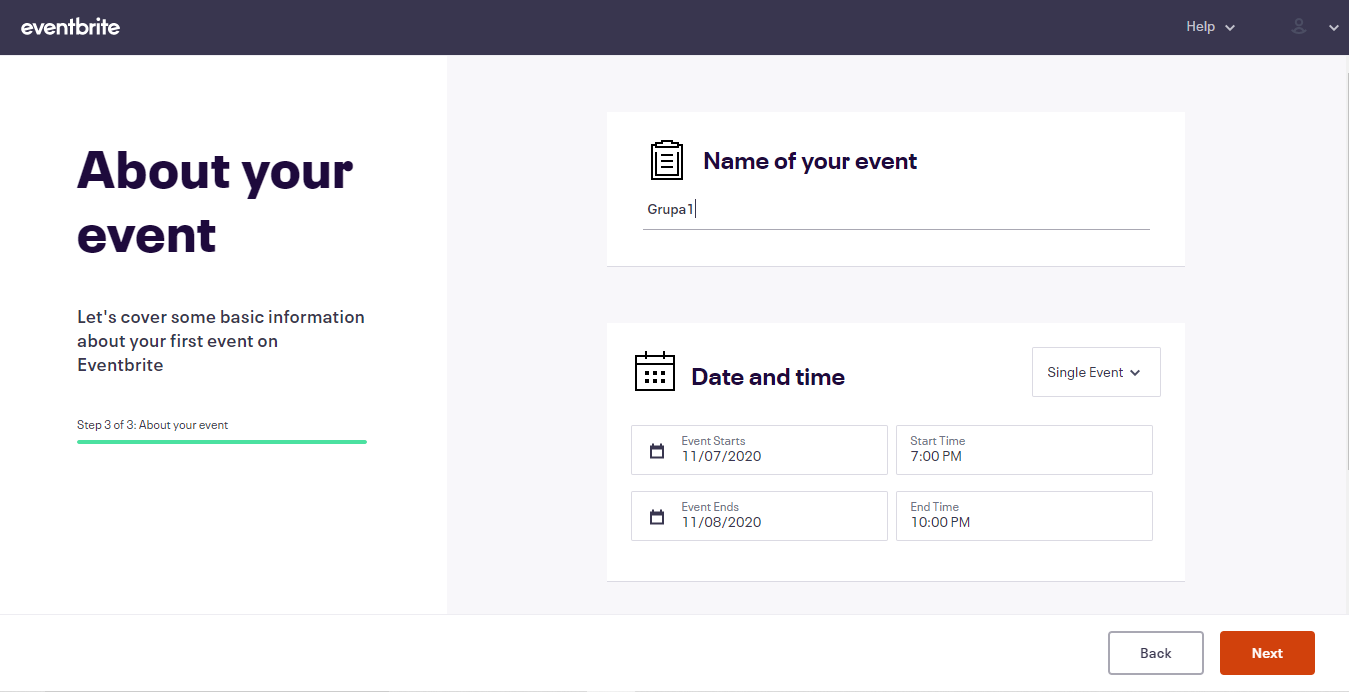
\includegraphics[width=.9\linewidth]{slike/eventbrite.png} %veličina u odnosu na širinu linije
			\centering
			\caption{Izgled \textit{eventbrite} forme pri pravljenju događaja}
			\label{fig:eventbrite} %label mora biti drugaciji za svaku sliku
		\end{figure}
		
		Postoje i alternative \textit{Eventbritu} slične kvalitete poput web stranice \textit{Billetto} dostupne na \url{https://billetto.co.uk/}. Ovaj servis dodatno omogućava korisnicima da pretražuju sve događaje dotad napravljene na toj stranici. Prednost takvog pristupa za organizatore je da im je time događaj dodatno reklamiran.
		
		\begin{figure}[H]
			
\includegraphics[width=.9\linewidth]{slike/billetto.png} %veličina u odnosu na širinu linije
			\centering
			\caption{Pretraživanje događaja na web stranici \textit{Billetto}}
			\label{fig:Billetto} %label mora biti drugaciji za svaku sliku
		\end{figure}
	
		Nadalje, slična funkcionalnostima, iako tematski nešto udaljenija je aplikacija \textit{Eventee} dostupna na \url{https://eventee.co}. Ova aplikacija osmišljena je kako bi pomogla organizacijama u stvaranju događaja i upravljanju njihovim sudionicima. Dodatno, aplikacija organizatorima šalje statističke podatke o događaju u stvarnom vremenu. 
		
		
		\begin{figure}[H]
			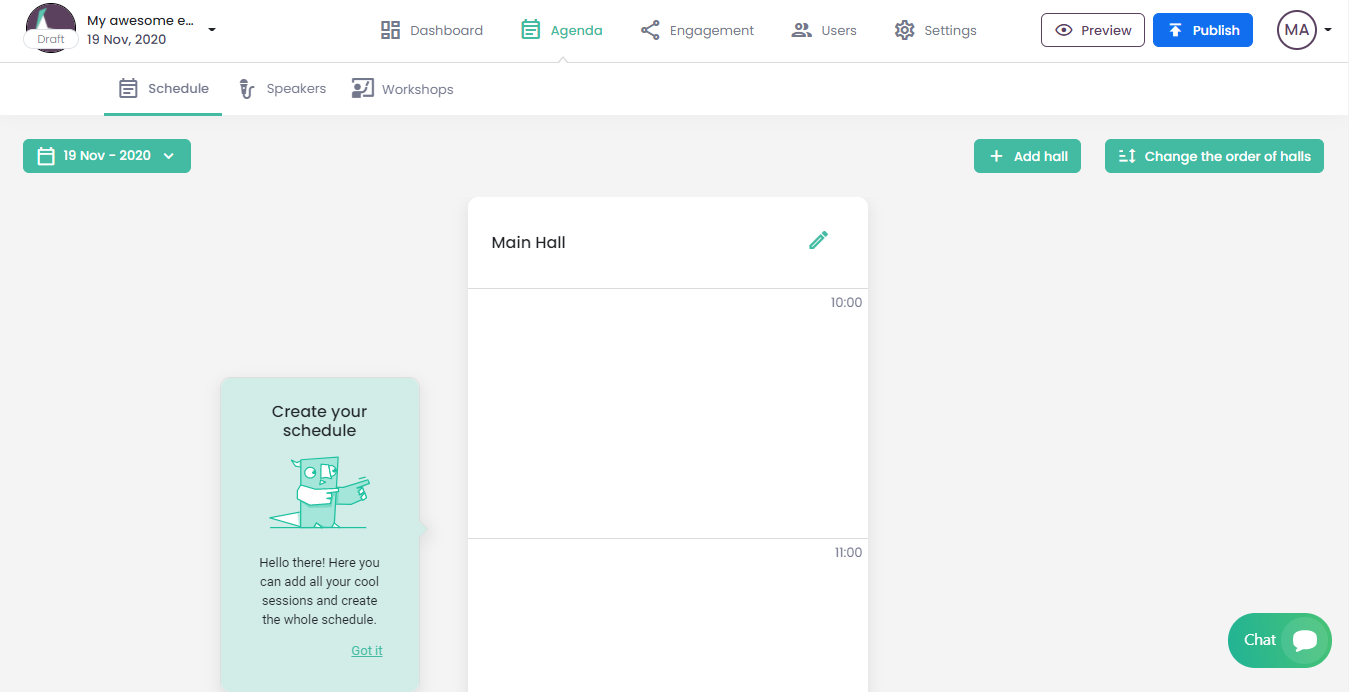
\includegraphics[width=.9\linewidth]{slike/eventee.png} %veličina u odnosu na širinu linije
			\centering
			\caption{Stvaranje novog događaja na web stranici \textit{Eventee}}
			\label{fig:eventee} %label mora biti drugaciji za svaku sliku
		\end{figure}
	
		Konačno, naveden je kratki pregled aplikacije \textit{Cvent} dostupe na \url{https://www.cvent.com}. Ova aplikacija nudi jednostavna i integrirana tehnološka rješenja kojima se nastoji maksimizirati učinak sastanaka i događaja različith veličina. Nastojanjem da povratnim informacijama o reakciji publike pomogne organizacijama u planiranju događaja kojima se cilja na određeno tržište, aplikacija se više orijentira na rješenja primjerena za događaje iz područja marketinga.  
		
		\begin{figure}[H]
			
\includegraphics[width=.9\linewidth]{slike/cvent.png} %veličina u odnosu na širinu linije
			\centering
			\caption{Početna stranica aplikacije \textit{Cvent}}
			\label{fig:cvent} %label mora biti drugaciji za svaku sliku
		\end{figure}
	
	
	
		
		\eject
		
		
		
		
	